\subsection{Simulations}

The list of Monte Carlo (MC) samples used as default in the presented analysis is given in Table \ref{tab:mc_samples1}. The dijet MC samples are produced in slices of $p_{T}$ of the original parton produced from the collision (and then sliced in truth anti-$k_t$ $R=0.6$ truth jet $p_T$).  These samples are reweighted to the correct $p_{T}$ spectrum in order to more efficiently populate the high tails of the $p_{T}$ distribution. The leading anti-$k_t$ R=0.4 jet distribution of the dijet MC sample is checked in Fig.\ref{fig:gbb-leadAkt4} to be smoothly falling to ensure the cross sections and samples weights are implemented correctly.

\begin{figure}[htbp]
  \centering
 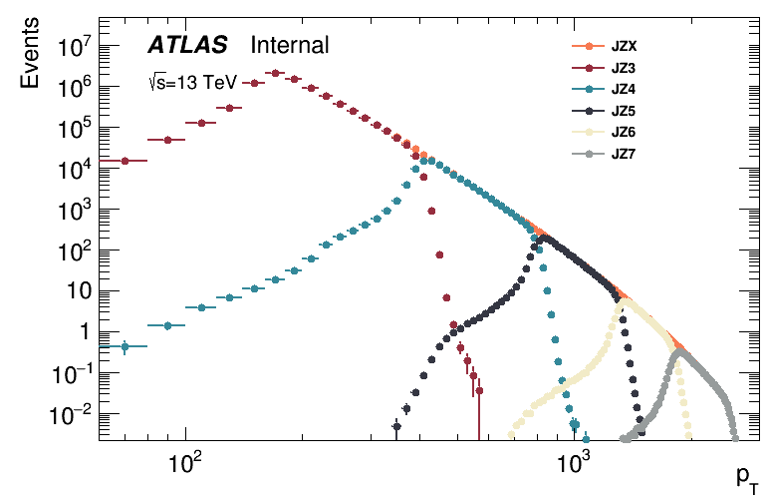
\includegraphics[width=0.4\textwidth]{figures/gbb/LeadJetCheck.png}
\caption{Distribution of $p_T$ of the leading anti-$k_t$ R=0.4 jet in each JZ slice and for all slices combined ``JZX''.}
  \label{fig:gbb-leadAkt4}
\end{figure}


\begin{table}[htpb]
\centering
\begin{tabular}{cccc}
Process & Name & ID & Generator \\
\hline 
\hline
Dijets & Pythia8\_EvtGen\_A14NNPDF23LO\_JZ3W & 361023 & Pythia  \\
Dijets & Pythia8\_EvtGen\_A14NNPDF23LO\_JZ4W & 361024 & Pythia  \\
Dijets & Pythia8\_EvtGen\_A14NNPDF23LO\_JZ5W & 361025 & Pythia  \\
Dijets & Pythia8\_EvtGen\_A14NNPDF23LO\_JZ6W & 361026 & Pythia  \\
Dijets & Pythia8\_EvtGen\_A14NNPDF23LO\_JZ7W & 361027 & Pythia  \\
\hline
\hline
\end{tabular}
\caption{Monte Carlo samples as used in the analysis. }
\label{tab:mc_samples1}
\end{table}


\subsection{Data}

The data samples used in this analysis were recorded by the ATLAS detector over the period June 2016 to December 2016, corresponding to data-taking periods A to L. This corresponds to an integrated luminosity of 33.1 fb${}^{-1}$ after application of basic data quality requirements via the standard ATLAS Good Run List\footnote{The official standard GRL for 2016 data (\url{data16_13TeV.periodAllYear_DetStatus-v83-pro20-15_DQDefects-00-02-04_PHYS_StandardGRL_All_Good_25ns.xml}) is used.}. The uncertainty on the integrated luminosity is 2.2\%. 

